% vim: spelllang=es

\chapter{Diseño}\label{sec:design}

\section{Arquitectura}

Para el sistema de plugins final, la estructura de Tremor debería ser la
ilustrada en la Figura~\ref{fig:separation}:

\begin{figure}
    \centering
    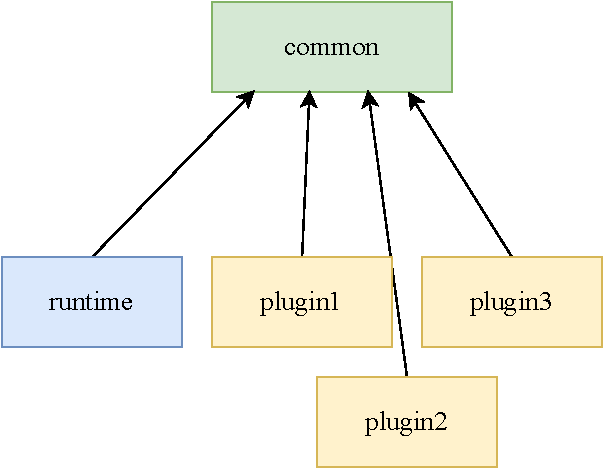
\includegraphics[width=7cm]{./Imagenes/separation.pdf}
    \caption{La estructura ideal para un sistema de plugins.}%
    \label{fig:separation}
\end{figure}

\begin{itemize}
    \item La \crate \code{runtime}, que carga los plugins.

    \item Las \crates \code{plugin}, con las implementaciones de los componentes
        del sistema.

    \item La \crate \code{common}, con la interfaz compartida entre la runtime y
        los plugins. Por tanto, ambos tipos de \crate dependen de \code{common}.

\end{itemize}

Esta estructura es esencial para el objetivo principal: mejorar los tiempos de
compilación. Existen dos maneras de entender los tiempos de compilación:

\begin{itemize}
    \item Para el desarrollo de la \textbf{runtime}

    \item Para el desarrollo de los \textbf{plugins}

\end{itemize}

En ambos casos, se quiere compilar únicamente \emph{uno} de los componentes. En
caso de desarrollar un plugin, no debería hacer falta recompilar también la
runtime, porque no está siendo modificada. Y si se está trabajando sobre la
runtime, no debería recompilarse la funcionalidad de los plugins.

El problema reside en que, inicialmente, únicamente existe una \crate con todo:
\code{runtime}, \code{plugin}s, y \code{common}. El primer paso debería ser el
que muestra la Figura~\ref{fig:separation_temporary}: separar los plugins del
mono-binario. La funcionalidad se encuentra en binarios diferentes, así que la
runtime tendrá un tiempo de compilación considerablemente menor. Desarrollar un
plugin también será menos costoso, ya que no hará falta compilar los demás.

\begin{figure}
    \centering
    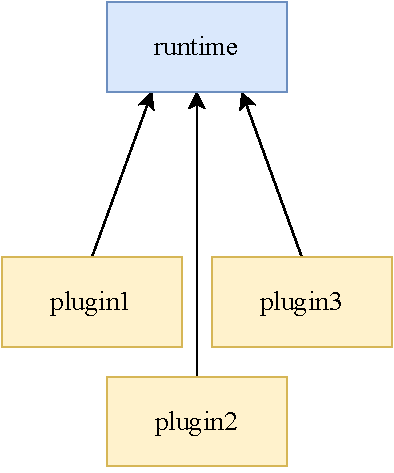
\includegraphics[width=6cm]{./Imagenes/separation-temporary.pdf}
    \caption{La estructura inicial del sistema de plugins para un desarrollo más
    rápido.}%
    \label{fig:separation_temporary}
\end{figure}

Para un tiempo de compilación óptimo también es necesario un segundo paso. La
interfaz del PDK sigue encontrándose en la misma \crate que la runtime, así que
un plugin tendrá que compilar también la runtime, aun cuando no es necesario.
Esto no será una mejora tan grande sobre los tiempos de compilación como en el
primer paso, dado que compilar la runtime es mucho menos costoso que compilar
todos los plugins.

Este segundo paso se puede omitir durante el inicio del desarrollo, ya que la
interfaz está muy fuertemente relacionada con la runtime. Los tipos usados en la
interfaz tendrán que moverse a una \crate distinta, pero todos estos tipos
provienen de la runtime, así que habrá que modularizar una gran parte del
código.

Cuantos menos cambios se produzcan al principio del proyecto, mejor. Habrán
menos conflictos y resultará más fácil y seguro revisar el ćodigo en pequeñas en
iteraciones, en vez de una única revisión grande.

\section{Plan de desarrollo}

A partir de la sección anterior, se puede elaborar un plan aproximado para el
sistema de plugins basado en iteraciones (o pull requests):

\begin{enumerate}
    \item \textbf{Definir una nueva interfaz y usarla internamente}: el sistema
        de plugins debería ser todo lo mínimo posible. La interfaz principal
        puede convertirse de forma que soporte plugins, pero se debería mantener
        todo en un mismo binario por simplicidad. La parte de cargado de plugins
        se puede dejar como una prueba de concepto por el momento y se pueden
        incluir algunos plugins externos para demostrar su funcionamiento.

        Esta iteración se podrá mergear con la rama principal, ya que el
        programa seguirá funcionando de la misma forma, simplemente con una
        interfaz distinta para los conectores internamente.

    \item \textbf{Realmente hacer los plugins externos}: dado que los plugins
        desarrollados usan la nueva interfaz, este paso debería ser sencillo.
        Únicamente implicará una gran cantidad de cambios, ya que implica
        reorganizar el repositorio con \crates nuevas, arreglar el sistema de
        compilación y similares.

    \item \textbf{Separar la runtime de la interfaz}: como se ha explicado, esta
        parte es menos importante pero puede implicar un gran número de cambios.
        Por tanto, únicamente al final se separará la interfaz a una crate
        \code{common} nueva, para una última mejora a los tiempos de
        compilación.

    \item \textbf{Otras mejoras para el despliegue}: últimos cambios antes de
        incluir el sistema de plugins en la nueva versión, incluyendo
        su documentación o la evaluación de los resultados finales.

\end{enumerate}

\section{Tecnologías a considerar}

Esta sección describe las tecnologías que se han considerado más viables como
base para el PDK. Algunas de ellas no cumplirán los requerimientos mencionados
al principio del capítulo, pero es necesario aprender sobre ellas primero antes
de escribir ninguna línea de código.

\subsection{Lenguajes interpretados}

Todo tipo de proyectos usan lenguajes interpretados para extender su
funcionalidad a tiempo de ejecución, como Python, Ruby, Perl, Bash, o
JavaScript. Particularmente, el editor de texto Vim creó su propio lenguaje para
poderlo personalizar por completo, Vimscript~\cite{vimscript}. Ahora NeoVim, un
fork más moderno, está esforzándose por tener Lua como lenguaje de primera clase
para su configuración~\cite{nvimlua}. Incluso Tremor tiene su propio lenguaje
para configurarlo, Troy.

% TODO: alguna traducción de 'embedding' decente?
De todos los lenguajes disponibles, Lua sería una de las mejores opciones para
este sistema de plugins en específico. Está hecho con \emph{embedding} en mente:
es simple y únicamente alrededor de 220KB~\cite{ierusalimschy2006programming}.
Algunas implementaciones del lenguaje, como LuaJIT, son extremadamente
eficientes y pueden ser viables hasta en escenarios de rendimiento
crítico~\cite{luajitperf}. Adicionalmente, las garantías de seguridad de Lua son
más fuertes que otros lenguajes, dado que no requiere \unsafe y que incluye una
\sandbox (aunque es ``delicado y difícil de configurar
correctamente'')~\cite{luasandboxes}.

Rust dispone de librerías como \cratelink{rlua}, con bindings para interoperar
con Lua. \code{rlua} en particular parece enfocar su interfaz en ser idiomática
y segura, que es un punto positivo para una librería fuertemente relacionada con
C. Por desgracia, parece estar semi-abandonada y fue reemplazada por
\cratelink{mlua}. Por lo general, el ecosistema de Lua en Rust no parece lo
suficientemente maduro para un proyecto como este; aún queda trabajo para
mejorar la estabilidad.

También sería posible usar uno de los lenguajes interpretados creados
específicamente para Rust: \textcite{cratesiogluon}, \textcite{cratesiorhai} o
\textcite{cratesiorune}. Usarlos posiblemente resulte en código más limpio y
simple. Sin embargo, su ecosistema todavía está en su infancia y ninguna de las
opciones son tan estables o seguras como lenguajes de programación de propósito
general. Rhai, el más usado, anunció su versión v1.0 en julio de 2021 y no
sobrepasa las 200.000 descargas, mientras que Lua fue creado en 1993 y es uno de
los 20 lenguajes más famosos, según el \textcite{tiobe}.

De cualquier manera, portar el código a este sistema de plugins sería un trabajo
excesivamente laborioso. Todos los conectores tendrían que reescribirse por
completo a un lenguaje distinto. Para un proyecto nuevo sería una alternativa
interesante, pero ciertamente no lo es en el caso de Tremor.

\subsection{WebAssembly}

\textcite{wasm}, también conocido como Wasm, es esencialmente un formato binario
abierto y portable. A diferencia de binarios normales, el mismo ejecutable Wasm
puede correr en cualquier plataforma, siempre y cuando exista una runtime que lo
soporte. Comenzó como una alternativa a JavaScript exclusiva a la web, pero ha
evolucionado con el tiempo y ahora es posible usarlo en el escritorio gracias a
\textcite{wasi}.

Los objetivos de Wasm son maximizar la portabilidad y seguridad, sin un coste de
rendimiento excesivo. Su diseño incluye una \sandbox para lidiar con programas
no fiables, como es el caso en sistemas de plugins, y apenas no requiere usar
\unsafe. Ya que puede ser compilado desde otros lenguajes como Rust o C, el
código existente en Tremor podría ser reusado (lo cual era imposible con
lenguajes de \scripting).

Existen dos runtimes principales para Rust: \textcite{wasmer} y
\textcite{wasmtime}. Ambas son implementaciones competitivas que se enfocan a
unos u otros casos de uso. Por lo general, Wasmer es más adecuado para embebirlo
en programas nativos, mientras que Wasmtime se centra en programas individuales
--- aunque los dos se pueden usar apara ambos casos~\cite{wasmwikiusage}.

% TODO: quizá esta footnote es innecesaria; podría llamarlo `intérprete` y ya.
WebAssembly todavía es una tecnología relativamente nueva, así que algunas
partes siguen bajo desarrollo continuo y necesitan mejoras, como en rendimiento.
En comparación a JavaScript, \textcite{jangda2019not} muestra resultados
mezclados al realizar pruebas de rendimiento. Depende principalmente del
compilador\footnote{Nos referimos también a la runtime como un
\emph{compilador}, dado que las implementaciones más eficientes y populares son
intérpretes \emph{Just-In-Time} (JIT), que transforman partes del código fuente
a código máquina.} y del entorno que se esté usando, variando desde mejoras en
velocidad de 1.67x en Chrome, a 11.71x con Firefox. Cuando se compara contra
código nativo, \textcite{libsodiumwasmperf} describe una varianza similar, donde
Wasmer es 2.47x más lento y con Wasmtime es 3.28x. En resumen, mientras que
WebAssembly es una solución más eficiente que algunos lenguajes de \scripting,
sigue sin llegar al nivel de binarios nativos, y posiblemente no sea lo
suficiente para este caso.

Esta tecnología es de las más adecuadas encontradas por el momento; su único
problema es el rendimiento. Tras implementar algún sistema de plugins en
miniatura, su usabilidad era excelente. Si fuera posible transferir datos entre
la runtime y el plugin sin tener que copiarlos, sería definitivamente la mejor
alternativa.

La especificación de WebAssembly define únicamente enteros y decimales como sus
tipos disponibles~\cite{wasmertypes}. Existen algunas maneras de tratar tipos no
triviales como estructuras o enumeraciones:

\begin{itemize}
    \item A través de la \textcite{wasminterfacetypes}. Esta define un formato
        binario para codificar y decodificar los nuevos tipos que define: tipos
        de números más especializados, caracteres individuales, listas,
        estructuras y enumeraciones. También especifica una lista de
        instrucciones para transformar los datos entre WebAssembly y el mundo
        exterior. Notar que esta propuesta no intenta definir una representación
        fija de, por ejemplo, una cadena de caracteres en Wasm; intenta permitir
        tipos de alto nivel agnósticos a su representación.

        Adicionalmente, las interfaces se pueden definir independientemente del
        lenguaje de programación que se esté usando, gracias al formato
        \code{witx}~\cite{witx}, como muestra la Figura~\ref{fig:witx_example}.

        El mayor problema de esta solución es que aún está en ``Fase 1'': aún
        necesita mucho trabajo y su especificación no es estable. Ninguna de las
        runtimes tienen soporte para esta propuesta
        aún~\cite{interfacetypeswasmtime}\cite{interfacetypeswasmer}. Tras
        fallar al intentar usarlo, esta opción fue descartada.

    \item La forma actualmente funcional pero imperfecta, con punteros y memoria
        compartida. El usuario debe construir y serializar el tipo complejo y
        después guardarlo en la memoria reservada para Wasm, a la que la runtime
        puede acceder directamente con punteros. Esto es lo que otros sistemas
        de plugins como Feather o Veloren
        hacen~\cite{featherpluginsystem}\cite{velorenpluginsystem}, así que es
        garantizado que funciona.

        No sólo requiere esto un paso de serialización y otro de deserialización
        y escribir y leer todos los datos de una memoria, sino que también es
        una tarea ardua y complicado de hacer correctamente. A nivel de
        rendimiento esto implicaría copiar los datos, así que no es algo que
        Tremor se pueda permitir.

    \item Otra opción que usan programas como Zellij~\cite{zellijpluginsystem},
        que usa un ejecutable de Wasm en vez de usarlo como una librería. Para
        cargarlo, lo ejecuta y usa \stdin y \stdout para los flujos de datos.
        Por desgracia, esto también requiere copiar datos, y tiene que
        descartarse.

\end{itemize}

\begin{figure}
    \centering
    \begin{minted}{lisp}
(use "errno.witx")

;;; Add two integers
(module $calculator
  (@interface func (export "add")
    (param $lh s32)
    (param $rh s32)
    (result $error $errno)
    (result $res s32)
  )
)
    \end{minted}
    \caption{Ejemplo de interfaz definida con \code{witx}.}%
    \label{fig:witx_example}
\end{figure}

\subsection{eBPF}

eBPF es ``a revolutionary technology with origins in the Linux kernel that can
run sandboxed programs in an operating system kernel''~\cite{ebpf}. Sin embargo,
de forma similar a WebAssembly, su uso se ha extendido a \emph{user-space}. eBPF
define una lista de instrucciones que pueden ejecutarse por una máquina virtual,
también como WebAssembly funciona.

Esta tecnología es prometedora, ya que a diferencia de WebAssembly, no es
necesario serializar o deserializar los datos o escribirlos a una memoria
intermedia. Ya que existe control completo sobre la máquina virtual, la runtime
podría implementar una \sandbox personalizada para comprobar las direcciones de
memoria de donde se lee o escribe para asegurarse de que se encuentran en el
rango permitiendo, siendo posible compartir una única memoria. La única
penalización en el rendimiento sería interpretar las instrucciones en vez de
ejecutar código nativo, pero técnicamente Tremor sí que podría usarlo.

El problema principal con eBPF es que su suporte es carente. La mayoría de sus
usuarios usan C y lo muestra la poca cantidad de tutoriales, guías, artículos o
incluso librerías disponibles para Rust. No es posible compilar Rust a
instrucciones eBPF de forma oficial y la única runtime disponible es
\cratelink{rbpf} y derivados como \cratelink{solana_rbpf}, ya que este primero
parece estar obsoleto. Además, supondría un esfuerzo mucho mayor que
WebAssembly, ya que también requeriría implementar una \sandbox personalizada.

\subsection{Comunicación Inter-Proceso}

Otra opción popular para sistemas de plugins es la \emph{Comunicación
Inter-Proceso}, que divide el programa en un cliente y un servidor en procesos
distintos. El cliente actuaría como runtime y estaría conectado a múltiples
servidores que proporcionan la funcionalidad. Se podría comparar con el
\emph{Language Server
Protocol}\footnote{\url{https://microsoft.github.io/language-server-protocol/}},
basado en JSON-RPC y usado por la mayoría de editores de texto para tener
soporte especializado para cualquier lenguaje de programación.

Una ventaja común para todos los métodos de esta familia es que, de forma
similar a WebAssembly, los plugins se podrán escribir en Rust, así que el código
existente se podría reusar. Además, ya que el cliente y servidor se dividirían
en múltiples procesos, serían más seguros por lo general; plugins defectuosos no
afectarían a la runtime de Tremor.

\subsubsection{Sockets}

Son los que peor rendimiento tienen de acuerdo a la Figura
\ref{fig:ipc_comparison1} y la Figura \ref{fig:ipc_comparison2}, pero también
son los más famosos, y consecuentemente, los más fáciles de usar. Los \sockets
son la misma tecnología usada en cualquier servidor para comunicarse con un
cliente y viceversa, por lo que hay una cantidad enorme de implementaciones
disponibles.

\begin{figure}
    \centering
    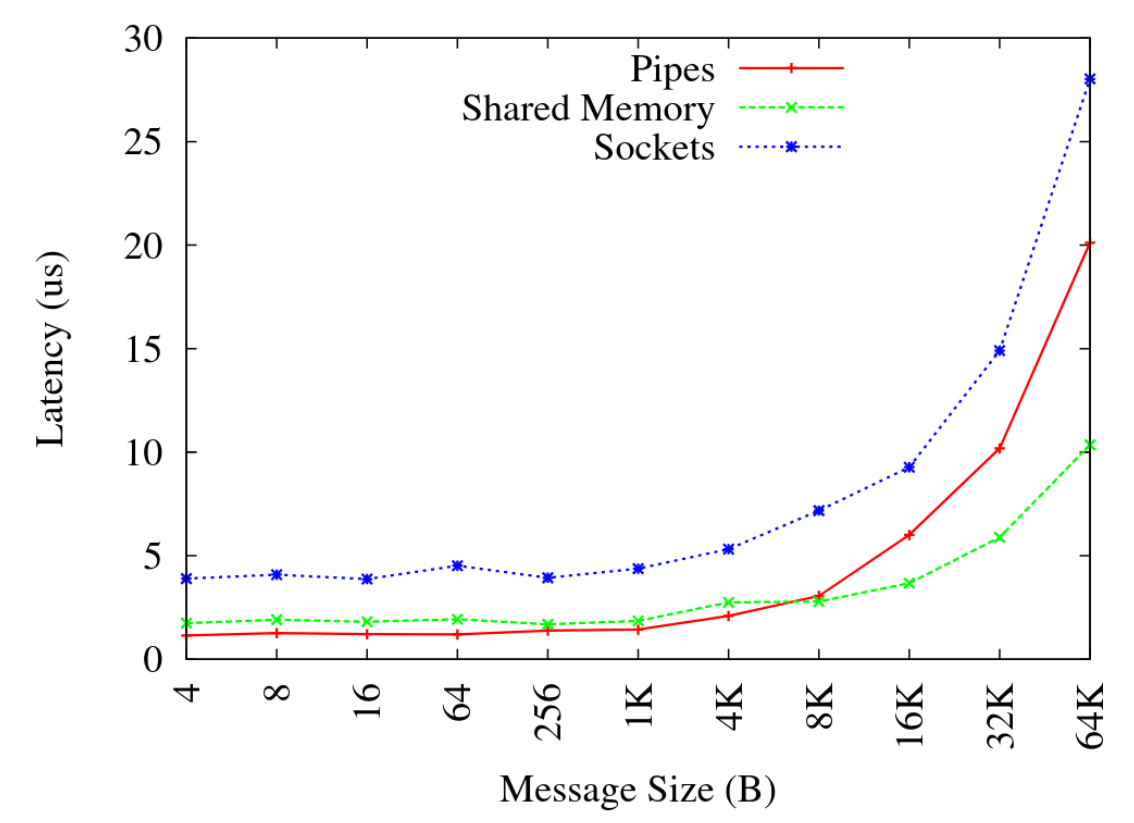
\includegraphics[width=12cm]{./Imagenes/venkataraman2015evaluation1.png}
    \caption{Latencia vs. Tamaño de Mensaje \cite{venkataraman2015evaluation}.}%
    \label{fig:ipc_comparison1}
\end{figure}

\begin{figure}
    \centering
    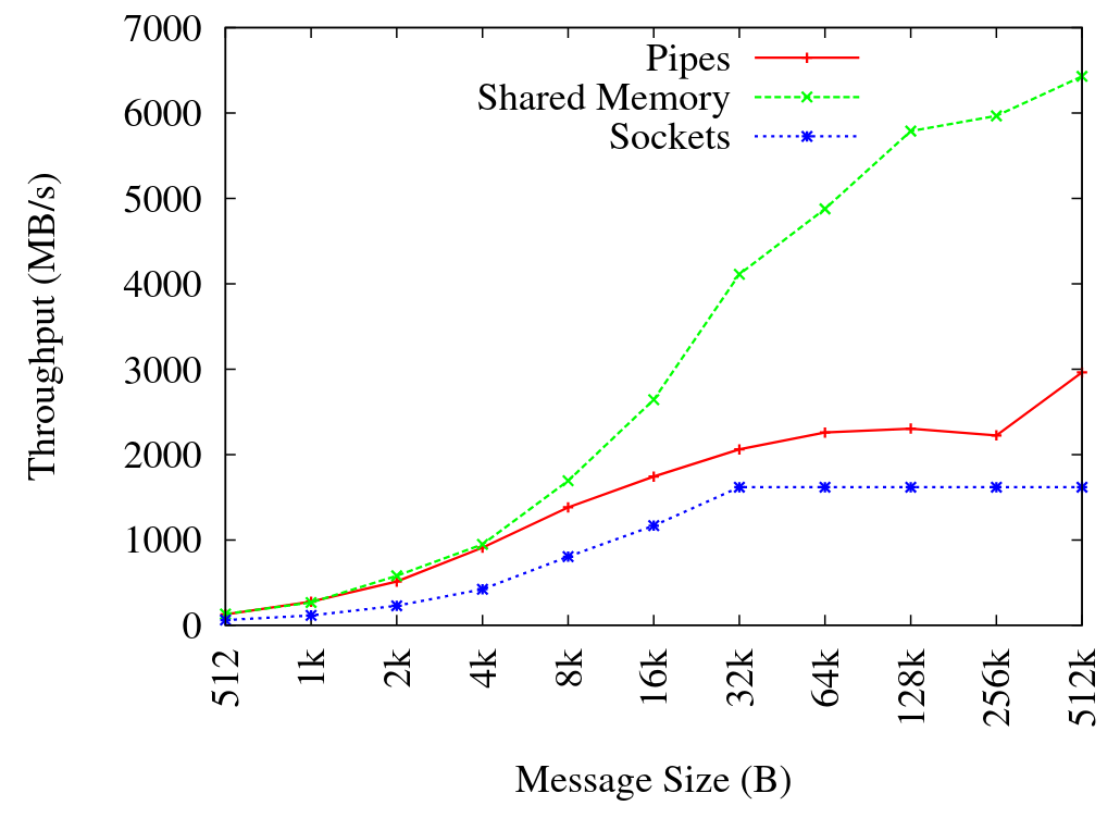
\includegraphics[width=12cm]{./Imagenes/venkataraman2015evaluation2.png}
    \caption{Rendimiento vs. Tamaño de Mensaje
    \cite{venkataraman2015evaluation}.}%
    \label{fig:ipc_comparison2}
\end{figure}

Usar \sockets también requiere un paso de deserialización, dado que los datos se
envían en paquetes. Formatos como JSON son los más flexibles, pero otros como
\textcite{protobuf} son ligeros y tienen mejor rendimiento.

\subsubsection{Pipes}

Para un sistema de plugins, las \pipes son muy similares a los \sockets, con la
única diferencia siendo que las \pipes solo se pueden usar en una misma máquina.
Con \sockets, técnicamente podrías usar TCP o UDP y tener la runtime y los
plugins en ordenadores distintos. Esto no es algo necesario para el caso de
Tremor, y ya que las \pipes ofrecen un mejor rendimiento, posiblemente sean una
mejor opción por lo general.

Por ejemplo, el gestor de archivos
nnn\footnote{\url{https://github.com/jarun/nnn}} usa este método: los plugins
pueden leer de una FIFO (una \pipe con nombre) para recibir las selecciones de
archivos o directorios que realice el usuario e implementar su funcionalidad
adicional.

La única desventaja es que no parecen haber librerías populares para la
funcionalidad genérica de \pipes (quizá \cratelink{interprocess} o
\cratelink{ipipe}). Sin embargo, esto podría ser innecesario si se usaran las
\pipes de \stdin, \stdout o \stderr implícitamente, ya que tienen soporte en la
librería estándar al ejecutar comandos \emph{shell}~\cite{rustpipes}.

\subsubsection{Memoria compartida}

Como el nombre indica, la memoria compartida consiste en inicializar un buffer
del que se puede leer y escribir desde dos o más procesos al mismo tiempo para
comunicarse. El API de memoria compartida se implementa a nivel del kernel, por
lo que depende mucho del sistema operativo y posiblemente no sea tan portable
como otras soluciones.

Tal y como indican las
Figuras~\ref{fig:ipc_comparison1}~y~\ref{fig:ipc_comparison2}, es el método con
mejor rendimiento, ya que no requiere copiar ni transformar datos entre
procesos. El único coste adicional es la inicialización de las páginas
compartidas en el sistema operativo, que se debe hacer únicamente al
principio~\cite{sharedmemperf}.

Desgraciadamente, el soporte para memoria compartida en Rust es casi
inexistente. Las únicas \crates disponibles son \cratelink{shared_memory} y
\cratelink{raw_sync}, que no superan las 150.000 descargas en total y usan gran
cantidad de \unsafe. Esto probablemente tenga que ver con el hecho de que
comparte los mismos problemas que cargado dinámico respecto a estabilidad de ABI
(explicado en la sección~\ref{sec:dynload}). No parece ofrecer nada mejor que el
cargado dinámico y por tanto se descarta como opción.

\subsection{Cargado dinámico}\label{sec:dynload}

Esta es la manera más popular para implementar un sistema de plugins, al menos
fuera de Rust. Una \emph{Foreign Function Interface} (FFI) nos permite acceder
directamente a recursos en objetos compilados separadamente, aun después de la
fase de \emph{linking}, gracias al cargado dinámico. Es una de las opciones más
eficientes porque no implica casi ningún coste adicinal tras cargar la librería
dinámica.

La \crate principal para este método es \cratelink{libloading}, aunque también
existen las menos conocidas \cratelink{dlopen} y \crate{sharedlib}, con pequeñas
diferencias~\cite{cratesdynloadcompare}. Todas ellas requieren de uso extensivo
de \unsafe, son complicadas de usar
correctamente~\cite{hardplugins1}\cite{hardplugins2}, incluyendo sutiles
disparidades entre sistemas operativos~\cite{hardplugins3}, ni disponen de un
mecanismo similar a una \sandbox. La única manera de mejorar la usabilidad será
a través de los macros y herramientas facilitados por algunas librerías.

\subsubsection{Estabilidad del ABI}\label{sec:abi}

El problema principal con esta alternativa es que Rust carece de un
\emph{Application Binary Interface} (ABI) estable. El ABI es una interfaz entre
dos módulos binarios, en nuestro caso entre un ejecutable (runtime) y una
librería dinámica (plugin). Este se encarga de definir, entre otros, la
estructura que siguen los tipos en memoria y la convención usada para llamar
funciones. Sin un ABI definido (y por tanto, \emph{estable}), sería imposible
saber cómo acceder a los recursos de otros binarios.

En el comienzo este proyecto, gran cantidad de fuentes en la comunidad
confundían cómo funciona este concepto en Rust, y lo explicaban de forma
incorrecta~\cite{wrongabi1}\cite{wrongabi2}\cite{wrongabi3}\cite{wrongabi4}.
Este popular malentendido también se dio en la propuesta del PDK y no nos dimos
cuenta del verdadero significado hasta haber invertido numerosas horas. El
equipo de Tremor --- yo incluido --- creía que el ABI de Rust es estable,
siempre que los dos binarios se compilen con la misma versión de compilador. Sin
embargo, esto es incorrecto por varias razones y fuentes como la referencia
oficial no entran en suficiente detalle~\cite[Application Binary Interface
(ABI)]{rustref}. Debe recurrirse a otra sección que menciona brevemente lo
siguiente:

``La estructura de tipos en memoria puede cambiar con cada compilación. En vez
de intentar documentar exactamente qué se hace, se documenta solo lo que se
garantiza hoy''~\cite[Type Layout]{rustref}

La asumpción anterior incorrecta se basa en que, hasta el momento, Rust no ha
implementado ninguna optimización que rompa el ABI entre ejecuciones de un mismo
compilador. Pero no existe absolutamente ninguna garantía de que esto sea así, y
es un detalle de implementación del compilador del que no debería confiarse. Es
posible que este comportamiento sí que se rompa en el
futuro~\cite{randomizelayout}, en cuyo caso el sistema de plugins tendría que
reescribirse por completo.

% TODO: a lo mejor lo de órdenes de magnitud se podría cambiar por algo mejor
Descubrir esto implicó un cambio de planes y un aumento en la complejidad del
proyecto de órdenes de magnitud. Ahora tendría que recurrirse a una ABI que sí
que tuviera garantías de estabilidad, y traducir entre la de Rust y esta para
comunicarse entre runtime y plugins. La ABI más conocida es la del lenguaje de
programación C, que se puede acceder desde Rust como indican las
Figuras~\ref{fig:rustpure}~y~\ref{fig:rustffi}.

\begin{figure}
    \centering
    \begin{minted}{rust}
pub struct Event {
    pub count: i32,
    pub name: &'static str,
}

pub fn transform(x: Event) -> i32 {
    println!("Received an event with count {}", x.count);
    x.count
}

pub static cached: Event = Event {
    count: 0,
    name: "my data"
};
    \end{minted}

    \caption{Ejemplo de cómo sería un plugin escrito con Rust.}%
    \label{fig:rustpure}
\end{figure}

\begin{figure}
    \centering
    \begin{minted}{rust}
// Using C's memory layout with `#[repr]`
#[repr(C)]
pub struct Event {
    // We can't have types from the standard library anymore, only
    // either basic ones...
    pub count: i32,
    // ...or types from C itself
    pub name: *const std::os::raw::char_c,
}

// Using C's calling conventions with `extern "C"`
pub extern "C" fn transform(x: Event) -> i32 {
    println!("Received an event with count {}", x.count);
    x.count
}

// Disabling mangling so that the resource's name is known when
// loading the plugin.
#[no_mangle]
pub static cached: Event = Event {
    count: 0,
    name: "my data".as_ptr() as _
};
    \end{minted}

    \caption{El mismo plugin que la Figura~\ref{fig:rustpure}, pero usando el
    ABI de C.}%
    \label{fig:rustffi}
\end{figure}

\subsubsection{Herramientas disponibles}

Todo este proyecto va a ser posible gracias a una \crate de más alto nivel,
\cratelink{abi_stable}. Esta usa \code{libloading} internamente y exporta una
gran cantidad de macros y herramientas para facilitar el desarrollo. Incluye una
copia de la librería estándar de Rust declarada con el ABI de C, generalmente
precedidos por la letra \code{R}. Por tanto, en vez de \rust{Vec<T>}, podremos
usar \rust{RVec<T>}; en caso contrario habría que recurrir a punteros
\rust{*const T} o tendríamos que reescribir los tipos desde cero nosotros.
También da soporte para librerías externas muy conocidas en la comunidad, como
\cratelink{crossbeam} o \cratelink{serde_json}. La
Figura~\ref{fig:rustabi_stable} demuestra parte de la simplificación del código
en la Figura~\ref{fig:rustffi}.

Existen algunas alternativas o extensiones de \abistable como
\code{lccc}\footnote{\url{https://github.com/LightningCreations/lccc}},
\cratelink{safer_ffi} o \cratelink{cglue} que se tuvieron en cuenta, pero no son
soluciones tan completas ni maduras, por lo que no serán incluidas en este
proyecto. \abistable se trata de una librería compleja, con más de 50.000 líneas
de código en Rust (como referencia, Tremor tiene unas 35.000 líneas), lo cual
deberá tenerse en cuenta en la decisión final también.

\begin{figure}
    \centering
    \begin{minted}{rust}
// Now we also "derive" the trait StableAbi, i.e., it's implemented
// automatically.
#[repr(C)]
#[derive(StableAbi)]
pub struct Event {
    pub count: i32,
    // We can use abi_stable's types!
    pub name: RStr<'static>,
}

// Using C's calling conventions with `extern "C"`
#[sabi_extern_fn]
pub fn transform(x: Event) -> i32 {
    println!("Received an event with count {}", x.count);
    x.count
}
    \end{minted}

    \caption{El mismo plugin que la Figura~\ref{fig:rustpure}, pero con
        \abistable. La declaración de la global \rust{cached} se omite por
        simplicidad.}%
    \label{fig:rustabi_stable}
\end{figure}

\section{Sistemas de plugins de referencia}

Otro punto de estudio importante es qué plugins ya hay existentes en Rust y cómo
se han realizado:

\begin{itemize}
    \item El mismo Cargo o
        \code{mdbook}\footnote{\url{https://github.com/rust-lang/mdBook}}
        implementan un sistema de extensiones a través de la línea de comandos.
        Añadir un subcomando nuevo es tan sencillo como crear un binario con un
        prefijo establecido (e.g., \code{cargo-expand}). Si está disponible en
        la variable de entorno \code{PATH} al ejecutar \code{cargo}, se podrá
        invocar al plugin con \code{cargo expand} también. Es una manera
        especialmente simple y creativa de usar \pipes con IPC, dado que usa
        \stdin y \stdout para comunicarse con la runtime.

    \item \code{zellij}\footnote{\url{https://github.com/zellij-org/zellij}} es
        un entorno de trabajo en el terminal con ``un sistema de plugins que
        permite crear plugins en cualquier lenguaje que compile a WebAssembly''.
        De forma similar al caso anterior, funciona un binario distinto para
        cada plugin y el ejecutable principal ejecuta el código en WebAssembly,
        comunicándose con \stdin y \stdout.

    \item \code{xi}\footnote{\url{https://github.com/xi-editor/xi-editor}} es un
        editor de texto moderno ahora abandonado. Usa RPC con mensajes JSON para
        comunicarse con plugins en procesos distintos~\cite{xiplugin}, método
        también usado en Visual Studio Code~\cite{vscodeplugin} o
        Eclipse~\cite{eclipseplugin}.

    \item \cratelink{bevy} es un motor de videojuegos prometedor cuyas
        prestaciones se implementan como plugins. En la mayoría de los casos, se
        cargan en tiempo de compilación, pero \rust{bevy::dynamic_plugin}
        da la posibilidad de hacerlo dinámicamente. \code{bevy} se basa en la
        falsa estabilidad del ABI explicado en la sección~\ref{sec:abi} y
        únicamente usa tipos definidos en Rust.

        Otras fuentes como \textcite{dynloading1} o \textcite{dynloading2}
        también intentan usar cargado dinámico para funcionalidades similares.
        Este último se trata de \cratelink{amethyst}, el predecesor de
        \code{bevy}, que acabó rindiéndose debido a la inestabilidad del
        ABI~\cite{dynloading_giveup1}\cite{dynloading_giveup2}.

\end{itemize}

\section{Elección Final}

Tras implementar varios sistemas de plugins en miniatura con las tecnologías más
prometedoras mencionadas en este capítulo, se tomó la decisión de usar cargado
dinámico con \abistable. Cada alternativa tiene sus puntos fuertes y sus puntos
flojos, como ilustra la Figura~\ref{fig:triangle}, pero ninguna de las demás
terminaron de cumplir los requisitos de rendimiento establecidos por el equipo
de Tremor.

Todas las tecnologías excepto cargado dinámico, eBPF o memoria compartida
requieren la copia de los datos en algún momento, algo que Tremor no se puede
permitir. De esas tres posibles soluciones, todas tienen que lidiar con
problemas con el ABI. La que mejor soporte tiene es cargado dinámico, así que
ese será el camino tomado.

\begin{figure}
    \centering
    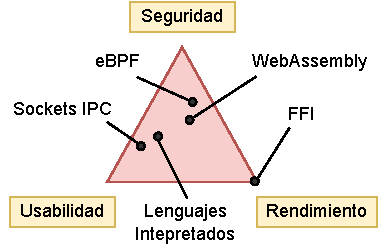
\includegraphics[width=10cm]{./Imagenes/triangle.pdf}
    \caption{Comparación aproximada de los métodos investigados.}%
    \label{fig:triangle}
\end{figure}
